% ============================== CHƯƠNG 6 ==============================
\chapter{Phân tích dự báo: Rủi ro trễ hạn trước khi giao hàng (Trang 3)}
\label{chap:predictive}

Chương này trình bày Feature~5 (\textit{Pre-Shipment ML Risk Scoring \& Driver Attribution})
và Feature~6 (\textit{What-If Order Delay Simulator}). Mã nguồn nằm trong thư mục \texttt{ml/},
chạy bằng \texttt{python run\_pipeline.py --step 7}.

% -----------------------------------------------------------------------------
\section{Phát biểu bài toán}
Cho một dòng đơn hàng tại thời điểm khách đặt hàng, dự báo xác suất
$P(\texttt{late\_delivery\_risk}=1)$, trong đó nhãn bằng 1 khi
\texttt{days\_shipping\_real} $>$ \texttt{days\_shipment\_scheduled}.
Grain là một order item (180.519 dòng, 65.752 đơn).

\subsection{Chống target leakage}
Chỉ dùng thông tin có tại thời điểm tạo đơn. Bảng~\ref{tab:leak-cols} liệt kê các cột bị loại.

\begin{table}[H]
\centering
\caption{Các cột bị loại để chống target leakage}
\label{tab:leak-cols}
\begin{tabularx}{\linewidth}{lX}
\toprule
\textbf{Cột} & \textbf{Lý do} \\ \midrule
\texttt{days\_shipping\_real}, \texttt{delay\_days}, \texttt{shipping\_date\_ts} & Chỉ biết sau khi giao; nhãn được suy ra trực tiếp \\
\texttt{delivery\_status} & ``Late delivery'' $\Leftrightarrow$ nhãn = 1 \\
\texttt{shipping\_ops\_key} & Junk dimension chứa \texttt{delivery\_status} \\
\texttt{order\_status} & CANCELED/SUSPECTED\_FRAUD $\Rightarrow$ nhãn luôn bằng 0 \\
\texttt{net\_profit}, \texttt{is\_loss\_order}, \ldots & Số liệu hậu kiểm \\
\bottomrule
\end{tabularx}
\end{table}

\subsection{Tập đặc trưng}
17 đặc trưng pre-shipment: 7 phân loại (\texttt{shipping\_mode}, \texttt{payment\_type},
\texttt{market}, \texttt{order\_region}, \texttt{customer\_segment}, \texttt{department\_name},
\texttt{category\_name}) và 10 số (\texttt{order\_hour}, \texttt{order\_dayofweek},
\texttt{order\_month}, \texttt{is\_weekend}, \texttt{is\_peak\_season},
\texttt{order\_item\_quantity}, \texttt{product\_price}, \texttt{discount\_rate},
\texttt{net\_sales}, \texttt{items\_in\_order}).

% -----------------------------------------------------------------------------
\section{Khám phá cơ chế sinh dữ liệu}
Phân tích phân phối số ngày giao thực tế (Hình~\ref{fig:dgp}) cho thấy:
\begin{itemize}
  \item \textbf{First Class} luôn giao sau đúng 2 ngày trong khi SLA là 1 ngày $\Rightarrow$ trễ 100\%.
  \item \textbf{Same Day}: đặt trước 12:00 giao trong ngày, đặt từ 12:00 trở đi giao ngày hôm sau $\Rightarrow$ trễ khi và chỉ khi \texttt{order\_hour} $\ge 12$.
  \item \textbf{Second} và \textbf{Standard Class}: số ngày giao thực tế phân phối đều trên $\{2,\dots,6\}$, độc lập với mọi đặc trưng khác $\Rightarrow$ tỷ lệ trễ cố định 80\% và 40\%.
\end{itemize}
Kiểm định chi-square trong từng nhóm Second/Standard cho thống kê xấp xỉ bậc tự do, và AUC
out-of-time của từng đặc trưng đơn lẻ nằm trong $[0{,}48;\,0{,}51]$, tức là không có tín hiệu.

\begin{figure}[H]
\centering
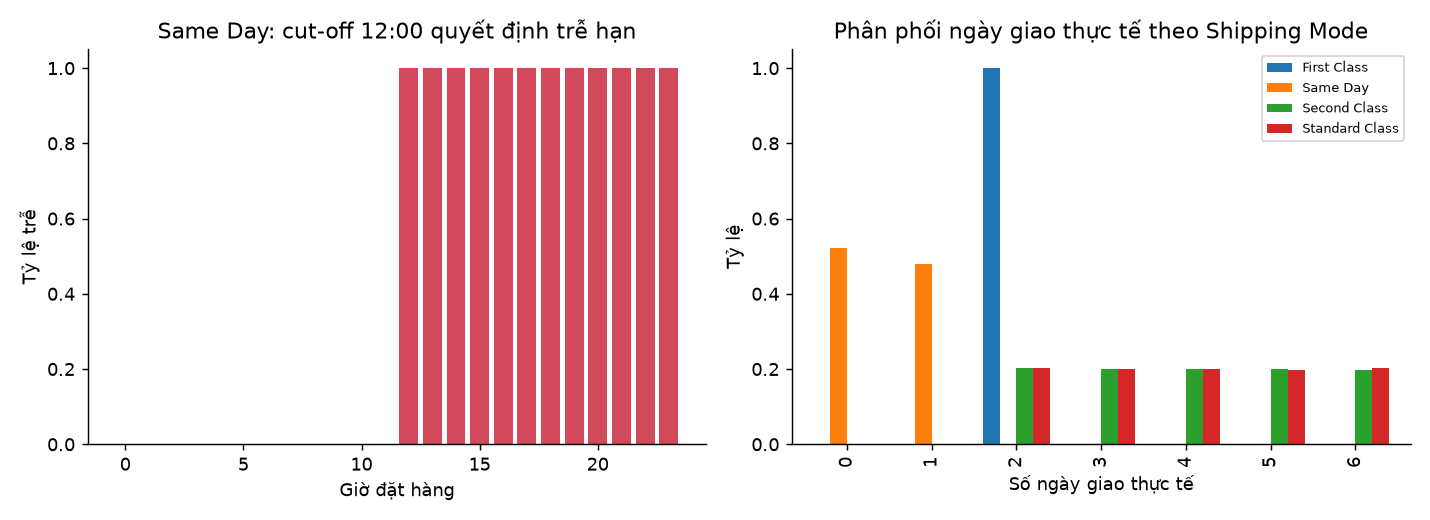
\includegraphics[width=\linewidth]{ml/06_data_generating_process.png}
\caption{Cut-off 12:00 của Same Day (trái) và phân phối ngày giao thực tế theo phương thức (phải)}
\label{fig:dgp}
\end{figure}

Từ đó xác định được \textbf{trần lý thuyết} (bộ phân loại Bayes):
\begin{equation}
P^*(\text{late}\mid x)=
\begin{cases}
1 & \text{First Class}\\
\mathbb{1}[\text{hour}\ge 12] & \text{Same Day}\\
0{,}8 & \text{Second Class}\\
0{,}4 & \text{Standard Class}
\end{cases}
\end{equation}
Mọi mô hình trung thực không thể vượt mức này một cách hệ thống; vượt quá đáng kể là dấu hiệu leakage.

% -----------------------------------------------------------------------------
\section{Thiết kế thực nghiệm}
\begin{itemize}
  \item \textbf{Out-of-time split:} train là các đơn trước 01/07/2017 (149.478 dòng), test là các đơn từ 01/07/2017 (23.287 dòng).
  \item \textbf{5-fold StratifiedGroupKFold} theo \texttt{order\_id} trên tập train: các item cùng đơn chung nhãn, nên phải chia theo nhóm.
  \item \textbf{Loại 7.754 đơn bị huỷ} khỏi train/eval (nhãn luôn bằng 0 bất kể phương thức).
  \item Tiền xử lý nằm trong sklearn \texttt{Pipeline}; chọn mô hình theo CV ROC-AUC, hoà thì theo CV Brier, không nhìn tập test.
\end{itemize}

% -----------------------------------------------------------------------------
\section{Kết quả}
\begin{table}[H]
\centering
\caption{So sánh mô hình trên tập test out-of-time (ngưỡng 0,5)}
\label{tab:model-cmp}
\small
\begin{tabular}{lrrrrcr}
\toprule
\textbf{Mô hình} & \textbf{Acc.} & \textbf{Prec.} & \textbf{Rec.} & \textbf{F1} & \textbf{ROC-AUC [95\% CI]} & \textbf{CV AUC} \\ \midrule
Baseline (tỷ lệ theo mode) & 69,90 & 89,13 & 54,45 & 0,676 & 0,750 [0,745--0,755] & 0,740 \\
Logistic Regression        & 70,98 & 89,44 & 56,33 & 0,691 & 0,754 [0,748--0,760] & 0,744 \\
\textbf{Decision Tree}     & \textbf{73,08} & \textbf{90,03} & \textbf{59,97} & \textbf{0,720} & \textbf{0,788} [0,782--0,792] & \textbf{0,774} \\
Random Forest              & 73,06 & 89,92 & 60,02 & 0,720 & 0,784 [0,778--0,789] & 0,771 \\
XGBoost                    & 72,41 & 86,59 & 61,71 & 0,721 & 0,783 [0,778--0,790] & 0,770 \\
LightGBM                   & 72,84 & 88,47 & 60,84 & 0,721 & 0,786 [0,781--0,792] & 0,771 \\ \midrule
\textit{Trần lý thuyết}    & \textit{73,08} & \textit{90,03} & \textit{59,97} & \textit{0,720} & \textit{0,781} [0,776--0,785] & \textit{0,774} \\
\bottomrule
\end{tabular}
\end{table}

\begin{figure}[H]
\centering
\begin{subfigure}{0.55\linewidth}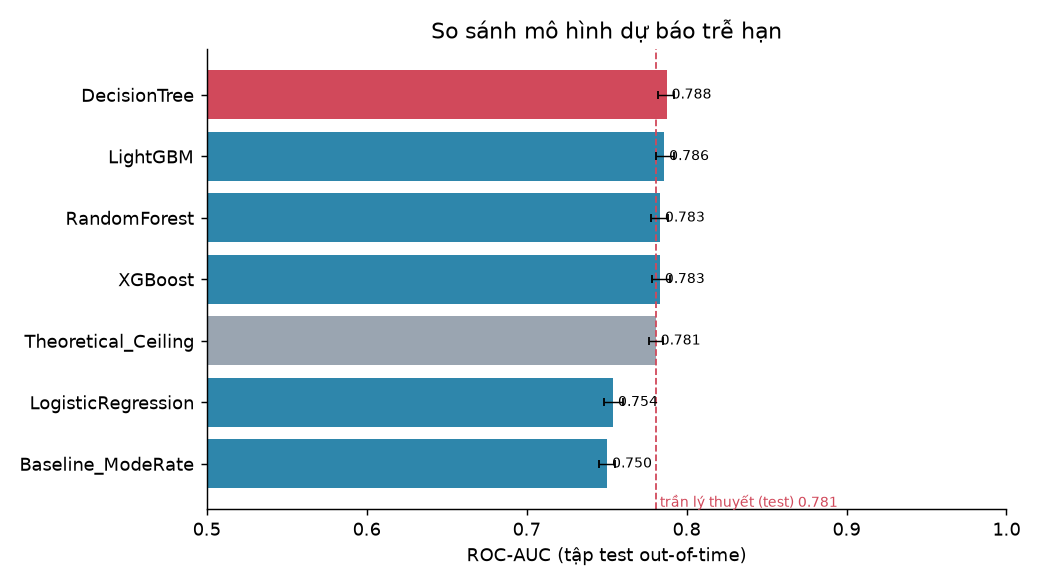
\includegraphics[width=\linewidth]{ml/01_model_comparison_auc.png}\caption{ROC-AUC kèm khoảng tin cậy}\end{subfigure}\hfill
\begin{subfigure}{0.42\linewidth}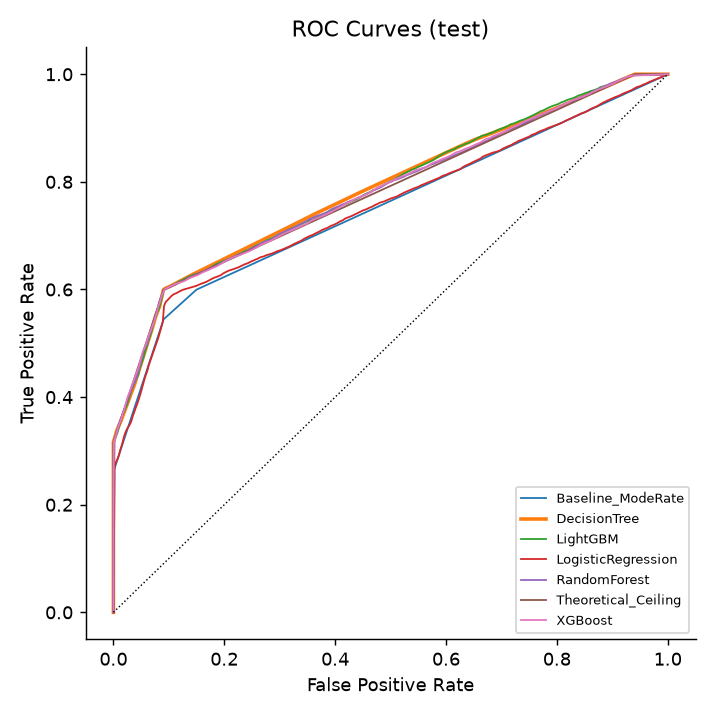
\includegraphics[width=\linewidth]{ml/02_roc_curves.png}\caption{Đường ROC}\end{subfigure}
\caption{So sánh hiệu năng các mô hình}
\label{fig:model-cmp}
\end{figure}

\paragraph{Diễn giải.}
\begin{enumerate}
  \item Các mô hình cây đều chạm trần lý thuyết. Decision Tree học đúng hai luật cốt lõi: First Class $\rightarrow$ trễ; Same Day và giờ $\ge 12$ $\rightarrow$ trễ. Các chỉ số tại ngưỡng 0,5 trùng khớp với trần.
  \item Logistic Regression kém hơn rõ rệt vì mô hình tuyến tính không học được tương tác \texttt{shipping\_mode} $\times$ \texttt{order\_hour}.
  \item Test AUC của mô hình cây nhỉnh hơn trần (0,788 so với 0,781) do dao động lấy mẫu: bên trong nhóm Standard và Second, AUC chỉ là 0,52 và 0,48. Trên CV của tập train, mô hình bằng trần (0,7743 so với 0,7736).
  \item Precision 90\% và Recall 60\%: cảnh báo ``trễ'' gần như luôn đúng, nhưng 40\% đơn trễ (chủ yếu Standard rơi vào kịch bản giao 5--6 ngày) không thể biết trước. Hạ ngưỡng xuống 0,40 thì Recall đạt 87\% và Precision 65\%.
\end{enumerate}

\begin{figure}[H]
\centering
\begin{subfigure}{0.48\linewidth}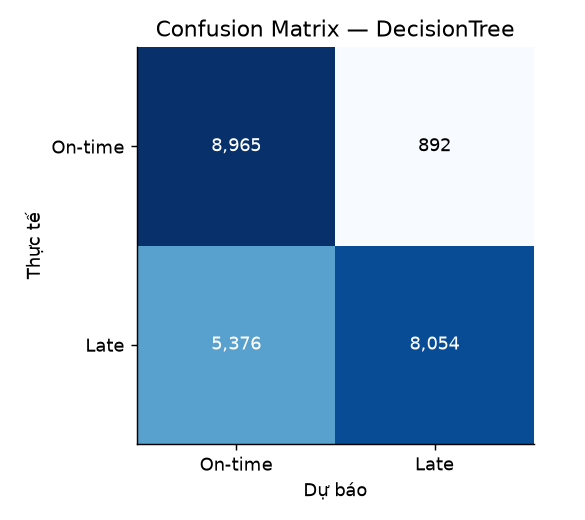
\includegraphics[width=\linewidth]{ml/03_confusion_matrix_best.png}\caption{Confusion matrix}\end{subfigure}\hfill
\begin{subfigure}{0.48\linewidth}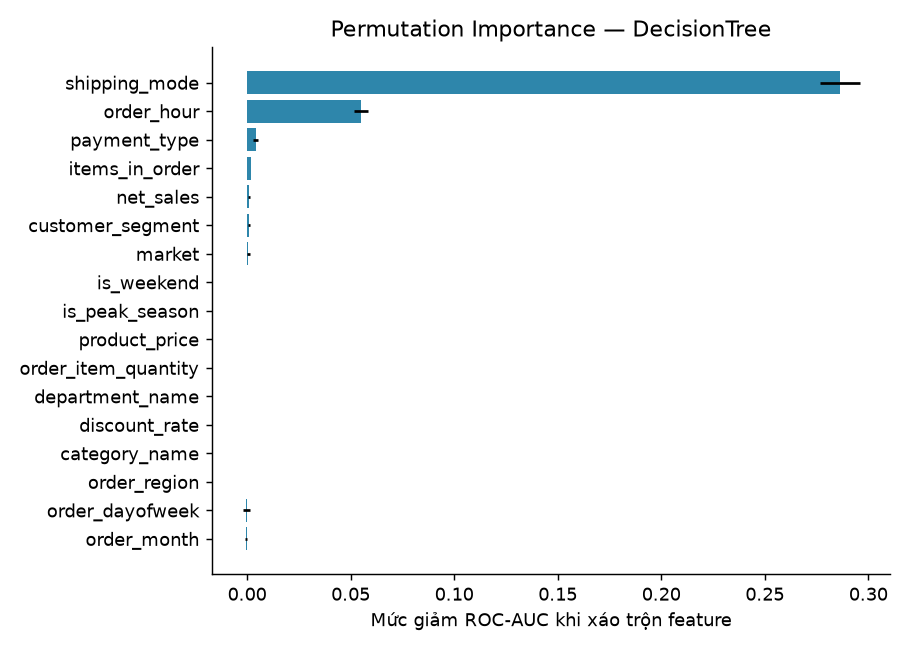
\includegraphics[width=\linewidth]{ml/04_feature_importance_best.png}\caption{Permutation importance}\end{subfigure}
\caption{Mô hình được chọn (Decision Tree)}
\label{fig:best-model}
\end{figure}

\paragraph{Yếu tố tác động.} \texttt{shipping\_mode} ($\Delta$AUC = 0,286) và \texttt{order\_hour}
(0,055) là hai yếu tố duy nhất có ý nghĩa; khu vực, ngành hàng và chiết khấu có $\Delta$AUC $<0{,}005$.
Điều này bác bỏ giả thuyết ``trễ do địa lý/sản phẩm'' và quy nguyên nhân về \textbf{chính sách SLA}.

\paragraph{Thí nghiệm leakage.} Thêm \texttt{days\_shipping\_real} vào đặc trưng cho AUC = 1,000 và
Accuracy = 100\%. Kết quả hoàn hảo nhưng vô dụng khi triển khai, minh chứng cho tầm quan trọng của
việc chọn đặc trưng pre-shipment.

% -----------------------------------------------------------------------------
\section{Feature 5 --- Dashboard đánh giá và chấm điểm rủi ro}
\todo{Chèn ảnh trang 3.1 và 3.2 vào \texttt{figures/dashboard/} và mô tả: slicer chọn mô hình, 7 KPI, ROC, importance, confusion matrix, slider ngưỡng; chấm điểm 180.519 vận đơn với 4 risk band, danh sách cảnh báo sớm.}

% -----------------------------------------------------------------------------
\section{Feature 6 --- What-If Order Delay Simulator}
Điều phối viên chọn 5 tham số (phương thức, giờ đặt, thị trường, chiết khấu, số lượng). Dashboard
tra lưới 14.400 kịch bản đã được mô hình chấm điểm trước, trả về xác suất trễ, risk band và
phương thức ít rủi ro nhất. Ví dụ: Same Day đặt lúc 14:00 có $P=100\%$, hệ thống gợi ý chuyển sang
Standard Class ($P=38\%$); đặt lúc 09:00 thì $P=0\%$.

Phần mô phỏng SLA tính tỷ lệ trễ kỳ vọng $P(\text{real days} > \text{SLA mới})$
(Bảng~\ref{tab:sla}), làm đầu vào cho Feature~8.

\begin{table}[H]
\centering
\caption{Kịch bản tái cấu trúc SLA (không tính đơn huỷ)}
\label{tab:sla}
\begin{tabular}{lccc}
\toprule
\textbf{Phương thức} & \textbf{SLA hiện tại $\rightarrow$ đề xuất} & \textbf{Trễ hiện tại} & \textbf{Trễ mới} \\ \midrule
First Class    & 1 $\rightarrow$ 2 & 100\%  & 0\% \\
Same Day       & 0 + cut-off 12:00 & 47,9\% & 0\% \\
Second Class   & 2 $\rightarrow$ 4 & 79,8\% & 39,8\% \\
Standard Class & 4 $\rightarrow$ 5 & 39,8\% & 20,2\% \\
\bottomrule
\end{tabular}
\end{table}
Áp dụng đồng thời bốn điều chỉnh, tỷ lệ trễ giảm từ 57,3\% xuống khoảng 19,8\% (OTD $\approx$ 80\%).
\todo{Chèn ảnh trang 3.3.}

% -----------------------------------------------------------------------------
\section{Hạn chế}
\begin{itemize}
  \item DataCo là dữ liệu bán tổng hợp: ngày giao của Second/Standard được sinh ngẫu nhiên đều, nên phần nhiễu này không thể khử bằng dữ liệu hiện có.
  \item Thiếu đặc trưng năng lực vận hành (hãng vận chuyển, tải kho, tuyến đường) vốn thường mang tín hiệu mạnh trong thực tế.
\end{itemize}
